\newpage
\begin{center}
\msyh 前言
\end{center}
\fsong
\par
随着数据中心服务器的增加,传统的系统维护方法有点捉襟见肘,于是出现了配置管理软件,利用配置管理,可以把整个数据中心的服务器的所有配置内容管理起来,方便大规模的管理以及快速的部署。配置管理软件有很多,最出名的是cfengine,但是cfengine的语法比较晦涩,于是出现了puppet  。puppet的语法简单,对管理内容的抽象很好,很容易理解代码,因此最近正迅速的流行开来。puppet是免费开源软件。可以自由使用,现在 google正使用puppet管理超过6000台的mac桌面电脑。这还是07年的数据。 另外很多世界知名的it企业也在使用puppet,开源社区的fedora也使用puppet。国内的大公司也在准备从cfengine转移到puppet上面。\par
撰写本文的目的是让初学者对 puppet有一个简单的认识能快速的入门,因为是利用空余时间完成,时间和精力有限,因此只讲解了最基本的内容,高级的内容都没讲解,如果你需要深入学习可以参考国内的中文 wiki 以及官方的文档。\par
本文欢迎转载,但是请保留作者信息。\par
本手册的最新版本可以从:http://code.google.com/p/puppet-manifest-share/downloads/list 获得。
\song
\newpage
\chapter{\msyh puppet简介}
\begin{center}
\kai
\small
滚滚长江东逝水,浪花淘尽英雄。是非成败转头空。\\
青山依旧在,几度夕阳红。 \\
白发渔樵江渚上,惯看秋月春风。一壶浊酒喜相逢。\\
古今多少事,都付笑谈中。\footnote{\fsong \tiny puppet被认为是下一代的cfengine,cfengine是一个老牌的配置管理软件}
\end{center}

\song
\section{\msyh puppet是什么}

puppet\footnote{\fsong\tiny 最开始是由luke开发的开源软件,现在开始公司化运作,但是软件依然是开源和免费的}是一个为实现数据中心自动化管理而设计的配置管理软件。基于c/s架构。puppet的服务器端保存着所有的对客户端服务器的配置代码,在puppet里面叫做manifest. 客户端下载manifest之后,可以根据manifest对服务器进行配置,例如软件包管理,用户管理和文件管理等等。
\par
这样就把日常的系统管理任务代码化了,代码化的好处是可以分享,保存,避免重复劳动,也可以快速恢复以及快速的大规模部署服务器。同时,manifest可以的根据客户端服务器的配置情况(硬件和软件)来动态生成。
\begin{center}
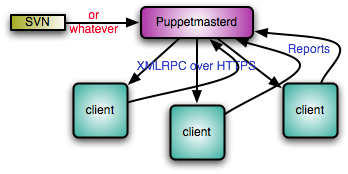
\includegraphics[width=0.6\textwidth]{Puppet_Star.png}
\end{center}


\par
在Unix/Linux系统管理的内容上面,通常就是管理软件包,用户,文件内容以及crontab等。在puppet的世界里面,这些内容都被看作是”资源“,每种资源都有对应的属性,例如软件包有安装和不安装的属性,文件有权限属性。puppet的代码主要就是由这些资源和资源的属性构成。
\par
为了快速的开始入门,建议你手上有一个可以随时使用的debian或者ubuntu系统,方便快速安装puppet软件。装一个虚拟机是一个不错的选择。\par

\section{\msyh Hello world}
puppet有两种执行模式,一是直接运行puppet file.manifest 二是puppetd --server puppetmaster.server.com;前面一种是直接读取file.mainfest文件进行配置,后一种是从服务端下载manifest进行配置。为了先对puppet的资源概念有一个简单的认识,下面将给出一个直接执行manifest的例子,看看manifest怎么去写。首先通过执行apt-get install puppet在系统上面安装好puppet客户端软件。然后编写一个manifest文件/tmp/1.pp,内容如下:
\msyh\small
\begin{lstlisting}
file {
      "/tmp/test":
        content=>"hello\n",
        mode => 0644;
        }
\end{lstlisting}
\song
然后执行 puppet  /tmp/1.pp ;执行完成以后,将会在/tmp目录下面生成一个文件test,文件内容是"hello";第一行的file表明是什么类型的资源,第二行的"/tmp/test"叫做这个资源的title;用来代表这个资源,后面两行设置这个资源的属性。\par
再来看一个例子:
\msyh
\begin{lstlisting}
package{
        ["gcc","make"]:
        ensure => installed;
}
\end{lstlisting}
\song
这是配置一个包资源,包是gcc和make, 第三行是指定这两个包的属性,在这里是installed,表示要安装这两个软件包。
\msyh 再次提醒:不同的资源有不同的属性,但是又有一些属性是所有资源都共有的,例如tag,这种属性叫做元属性。
\song
\newpage


